\chapter{Real-valued Optimization Algorithms}
\label{chapter:algos}

A real-valued optimization algorithm minimize a given \textit{objective function} in the continuous domain.
It searches the continuous domain by iteratively asking for the fitness of solutions.
We often evaluate an algorithm by the \textit{number of function evaluations} it consumes to obtain the global optimum solution.
This task is often described as the \textit{black box optimization},
since the algorithm has no prior knowledge about the problem characteristics or structures.
That means the gradient information might not be useful or even not available, so hill-climbing algorithms do not work.
The problem may be non-convex, multimodal, noisy and discontinuous.
In order to solve these kinds of problems, different algorithms have different assumptions about the problem structure.
They also use different stochastic models and update methods to try to converge to the global optimum as fast as possible.
These algorithms are often used for parameter and model calibration.  
The following section describes three kinds of milestone evolutionary algorithms 
that are commonly used as the baseline for real-valued optimization.


\section{Covariance Matrix Adaptation Evolution Strategy}
The \textit{Evolutionary Strategies} (ES) samples new search points with a normal distribution.
Each $d$-dimensional sample $x_i$ in a population with size $\lambda$ is drawn from a multivariate normal distribution as following:  
\begin{displaymath}
x_i \sim m + \sigma N_i(0,C),
\end{displaymath}
where $m \in \mathbb{R}^d$ is the mean, $\sigma \in \mathbb{R}_+$ is the step-size, and $C \in \mathbb{R}^{d \times d}$ is the covariance matrix.
The mean vector represents the positions where the best solution is most likely to appear.
The step-size determines the area to search and modifies exploration and exploitation behaviors.
The covaraince matrix determines the shape of the distribution ellipsoid.

\begin{figure}
\centering
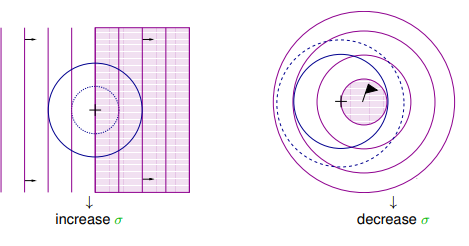
\includegraphics[width=\textwidth]{one_plus_one_ES}
\caption{The one fifth rule of (1+1)-ES.}\label{fig:one_plus_one_ES}
\end{figure}

\subsection{(1+1)-ES}
One of the simplest Evolutionary Strategy is \textbf{(1+1)-ES}.
It samples one offspring $x$ from parent $m$ according to the equation described above.
If the offspring $x$ is better than $m$, it replaces $m$ to be the new mean of the next sampling distribution.
It also follows the \textit{one-fifth success rule} as illustrated in Figure~\ref{fig:one_plus_one_ES}.
The one-fifth success rule increases the step-size by $1.5$ if the current sample is not better than the previous best sample, \textit{i.e.} the mean $m$.
We believe the best solution, denoted as the flag in Figure~\ref{fig:one_plus_one_ES}(a), 
should be somewhere outside of our current distribution and we should increase step-size to explore more search space.
The one-fifth success rule decreases the step-size by $1.5^{-1/4}$ if the current sample is better than the previous best sample.
This means that we believe the best solution, illustrated as the flag in Figure~\ref{fig:one_plus_one_ES}(b),
should be within the sampling distribution, and we should decrease the step-size to further focus on the current region.
Here we describe the (1+1)-ES with one-fifth success rule with independent restarts~\cite{Auger:2009:one_plus_one_ES}.
The pseudo code of (1+1)-ES is given in Algorithm~\ref{algo:1+1ES}.

\begin{algorithm}%[t!]
\caption{(1+1)-ES with 1/5 success-rule}\label{algo:1+1ES}

$\boldsymbol{X}_{n}$: solution of the $n^{th}$ iteration, $\sigma_n$: step size of the $n^{th}$ iteration, \\
$N(\boldsymbol{0}, \boldsymbol{I})$: multivariant normal distribution with mean vector $\boldsymbol{0}$ \\ 
and identical covariance matrix $\boldsymbol{I}$.

\BlankLine
\SetKwInOut{Input}{input} \SetKwInOut{Output}{output}
\Input{ $f$: evaluation function }
\Output{ $X_{n+1}$: best solution }

\BlankLine
Initialize $\boldsymbol{X}_0, \sigma_0$ \\
\While{ termination criterion not met } {

    $\widetilde{\boldsymbol{X}}_n = \boldsymbol{X}_n + \sigma_n N(\boldsymbol{0}, \boldsymbol{I})$  \\

    \eIf{ $f(\widetilde{\boldsymbol{X}}_n) \leq f(\boldsymbol{X}_n) $}{
        $\boldsymbol{X}_{n+1} = \widetilde{\boldsymbol{X}}_n$ \\
        $\sigma_{n+1} = 1.5 \sigma_n$
    }{
        $\boldsymbol{X}_{n+1} = \boldsymbol{X}_n$ \\
        $\sigma_{n+1} = 1.5^{-1/4}\sigma_n$
    }
}

\Return $\boldsymbol{X}_{n+1}$

\end{algorithm}



\subsection{CMA-ES}
Covariance Matrix Adaptation Evolution Strategy (CMA-ES) is an Evolutionary Strategy 
proposed by Hansen in 2003~\cite{Hansen:2003:CMA_ES}.
It adopts a multivariate normal distribution to generate \textit{isotropic} search points which do not favor any direction.
The multivariate normal distribution is widely observed in the nature and relatively easy to design and analysis for algorithms.
CMA-ES modifies three parameters to control the multivariate normal distribution: 
the mean $m \in \mathbb{R}^d$, the step-size $\sigma \in \mathbb{R}_+$, and the covariance matrix $C \in \mathbb{R}^{d \times d}$.


The \textit{mean} indicates the translation of the normal distribution model.
It indicates the most favorable position that should be sampled with the largest density.
It is updated with the weighted mean of all the positions according to their fitness.
The \textit{step-size} controls the state of exploration or exploitation.
An ideal step-size control gradually decreases the searching region for exploitation.
One of the easiest step-size control method is the one-fifth success rule, mentioned above.
Later a cumulative step-size adaptation is proposed in 
Cumulative Step-size Adaptation Evolutionary Strategy (CSA-ES)~\cite{Hansen:2001:CSA_ES}, a predecessor of CMA-ES.
The cumulative step-size adaptation measures the pathway of the mean vector in the generation sequence.
Adapting the step-size according to the \textit{evolution path} enables translating more efficiently to a desired location.
Later, it also allows perpendicular around the desired region.
The \textit{covariance matrix} indicates the shape of the normal distribution model.
Adapting the covariance matrix allows us to search in a region that is more coherent to the fitness landscape, 
This adaptation follows a natural gradient towards the direction of optimum solution.
It can also learn a rotated representation of the problem and be coordinate independent. 
By adjusting these three parameters, shown in Figure~\ref{fig:CMA_elements}, CMA-ES is extremely powerful on solving unimodal problems.

\begin{figure}
\centering
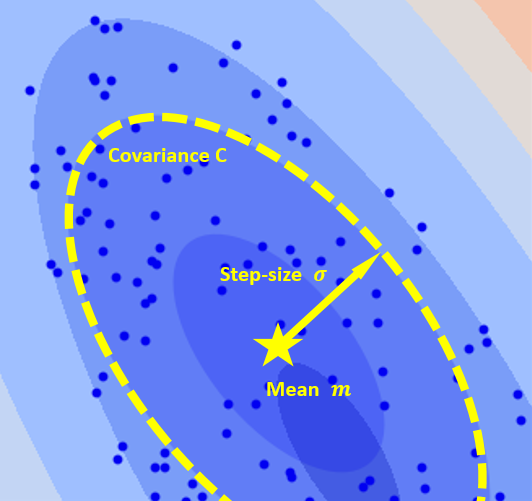
\includegraphics[width=4in]{CMA_elements}
\caption{Three major elements of CMA-ES.}\label{fig:CMA_elements}
\end{figure}

CMA-ES adopts a small \textit{population size} to reduce function evaluations and increase the frequency of updating the underlying models.
The default population size $\lambda$ for a $D$-dimension problem, described in~\cite{Hansen:2006:CMA_ES_review}, is
\begin{displaymath}
\lambda = 4 + \lfloor 3 \log(D) \rfloor .
\end{displaymath}
However, recent research suggest that it is benefitial to gradually increase the population size after random restart~\cite{Auger:2005:IPOP_CMAES}.
This parameter-less adaptation enables few evaluations consumption for easy problems, 
yet is also able to solve more difficult problems with a larger population size later.





\section{Standard Particle Swarm Optimization}

Particle Swarm Optimization (PSO) is a swarm intelligence optimization algorithm. 
%The swarm intelligence family... 
It was first proposed by J. Kennedy and R. C. Eberhart in 1995~\cite{Kennedy:1995:PSO} to simulate the foraging behavior of bird flocks.
The swarm is composed of \textit{particles} that move around in a given multi-dimensional \textit{search space} to find the best solution.
Each particle updates its velocity according to its historical experience, as well as the information of the neighboring particles.
The neighborhood of a particle is a set of information links defined by the \textit{swarm topology}. %, which indicates whom informs whom.
PSO iteratively updates the swarm topology, the velocities, and the positions of each particle until the global optimum solution is found.


Throughout the years, numerous variants of PSO have been proposed to improve performance.
As a result, a \textit{standard} PSO, composed of clear principals, is needed as the baseline for comparison.
Standard PSO (SPSO) provides a well defined version that follows the common principals of PSO design.
It is intended to be a milestone with simple and clear implementation for future comparison. %, instead of the best algorithm on the market.
So far, there have been three successive versions of standard PSO: SPSO 2006, SPSO 2007, and SPSO 2011.
The underlying principals of these three algorithms are generally the same as all PSO variants.
The exact formula and implementation are slightly different due to latest theoretical progress.
A detailed description of SPSO 2011~\cite{Zambrano:2013:SPSO2011} is given in the following paragraphs.

\subsection{Initialization of the swarm}

For a search space $E$ with a given dimension $D$, $E$ is confined by a set of minimum and maximum bounds in each dimension.
The hyperparallelepid search space $E$ can be formally defined as the Euclidean product of $D$ real intervals~\cite{Clerc:2012:SPSO2011}:
\begin{displaymath}
E = \bigotimes_{d=1}^{D}[min_d, max_d].
\end{displaymath}
For each position $x$ within the multi-dimensional search space $E$, there exists a corresponding numerical value $f(x)$, \textit{i.e.} \textit{fitness}.
A swarm is composed of particles, which explore different positions in the search space to find the best corresponding fitness value.
At time $t$, each particle in the swarm possesses the following vectors with $D$ coordinate:
\begin{itemize}
\item $x_i(t)$ is the \textbf{position} of the particle $i$ at time $t$.
\item $v_i(t)$ is the \textbf{velocity} of the particle $i$ at time $t$.
\item $p_i(t)$ is the \textbf{previous best position} the particle $i$ had been to, at time $t$.
\item $l_i(t)$ is best position of all the previous best positions in the \textbf{neighborhood} of particle $i$ at time $t$.
\end{itemize}

Let $U(min_d, max_d)$ be a random number drawn from a uniform distribution within $[min_d, max_d]$, 
and $N_i(t)$ be a set of neighbors of particle $i$ at time $t$ defined by the swarm topology.
In SPSO 2011~\cite{Clerc:2012:SPSO2011}, each particle is initialized with a random position and velocity defined as following:
\begin{align*}
x_i(0) &= U(min_d, max_d), \\
v_i(0) &= U(min_d - x_{i,d}(0), max_d - x_{i,d}(0)), \\
p_i(0) &= x_i(0), \\ 
l_i(0) &= argmin_{j \in N_i(0)}(f(p_j(0))).
\end{align*}


%The swarm size, denoted as $S$, differs in SPSO 2006 and SPSO 2011.
%In both SPSO 2006 and SPSO 2007, the initial number of particles $S$ for dimension $D$ is defined as:
%\begin{displaymath}
%S = 10 + \lfloor 2\sqrt{D} \rfloor,
%\end{displaymath}
%However, emperically, the definition of swarm size in SPSO 2006 is far from optmial swarm size~\cite{Clerc:2012:SPSO2011}.
%Therefore, in SPSO 2011, the swarm size is suggested as
The swarm size of SPSO 2011, denoted as $S$, is suggested as
\begin{displaymath}
S = 40,
\end{displaymath}
yet it can also be defined by user~\cite{Clerc:2012:SPSO2011}.


\subsection{Velocity update equations}

Velocity update equations differs in different variations of PSO, 
since it is the core procedure of optimization that determines the performance of PSO.
To prevent premature convergence, 
SPSO follows a random permutation order to update the positions of particles in the swarm~\cite{Clerc:2012:SPSO2011}.
The position of particle $i$ at time $t+1$ depends on the previous position and the current velocity:
\begin{displaymath}
x_i(t+1) = x_i(t) + v_i(t+1).
\end{displaymath}
The velocity of particle $i$ at time $t+1$ can be described as a combination of three vectors:
\begin{displaymath}
v_i(t+1) = w v_i(t) + \alpha (p_i(t) - x_i(t)) + \beta (l_i(t) - x_i(t)),
\end{displaymath}
where $w$ mimics the momentum of the particle, and $\alpha$, $\beta$ describes how successive actions are effected by the personal previous best position and the neighborhood previous best position.

%In SPSO 2006 and SPSO 2007, the velocity update equation is applied dimension by dimension as follows:
%\begin{align*}
%v_i(t+1) &=  w v_i(t) + U(0,c)(p_i(t) - x_i(t)) + U(0,c) (l_i(t) - x_i(t)) \\
%       w &= \frac{1}{2\ln(2)} \simeq 0.721 \\
%       c &= \frac{1}{2} + \ln(2) \simeq 1.193
%\end{align*}

%Figure~\ref{fig:SPSO_update} visualize the three main vectors in a two dimensional problem.
%The first part, $v_1$, represents the influence of previous action on current velocity.
%$w$ is the inertia weight that resembles the momentum, relating the next velocity to the latest velocity $v_i(t)$.
%It allows \textit{exploration} by giving a tendency of expanding the search space.
%The second part, $v_2$ is a random vector drawn from the parallelepid $c(p_i(t) - x_i(t))$.
%$c$ is the acceleration constant and the parallelepid $c(p_i(t) - x_i(t))$ represents the effect of personnal best memory $p_i(t)$ on current decision making.
%The third part, $v_3$ is a random vector drawn from the parallelepid $c(l_i(t) - x_i(t))$
%The parallelepid $c(l_i(t) - x_i(t))$ mimics how the best social memory $l_i(t)$ contributes to current decision making.
%The last two parts allows \textit{exploitation}, by attracting the particles near the possible optimum positions.
%Therefore, the new velocity depends on the latest action, personnal best memory, and social influence.

%However, the velocity update equations of SPSO 2006 depends on the system of coordinates.
%The distribution of all possible next positions is more dense near the center of a $D$ dimension rectangle.
%Moreover, the dimension-by-dimension updating method makes the algorithm dependent to system coordinates.
%It is extremely easy to find the optimum point lying on an axis, a diagonal or the center of the coordinate.

\begin{figure}[!t] \centering
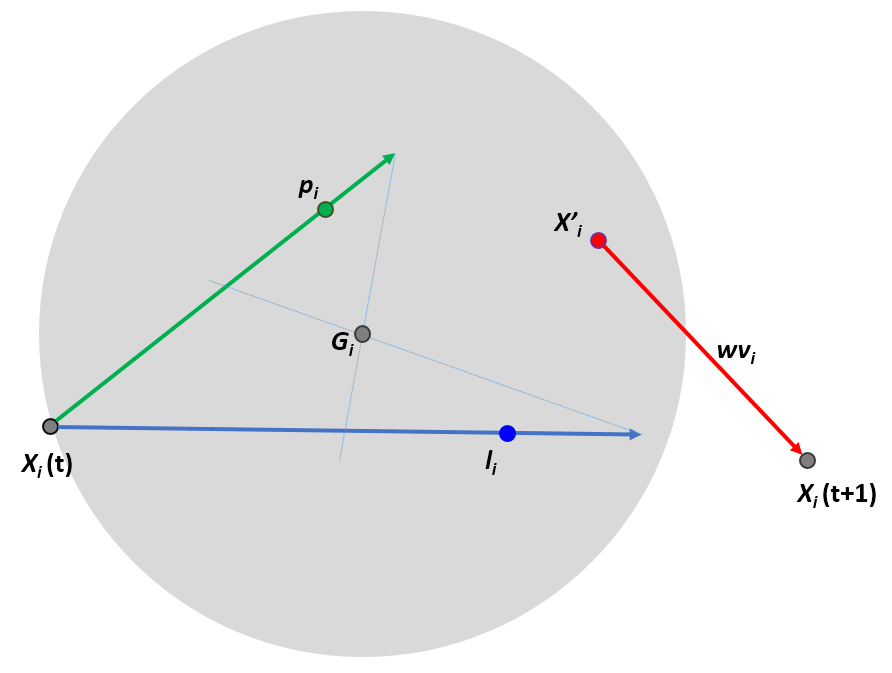
\includegraphics[width=4.5in]{SPSO_2011}
\caption{Velocity update of SPSO 2011.}\label{fig:SPSO_2011}
\end{figure} 


In SPSO 2011, the velocity update equations eliminates the coordinate dependency by creating a hypersphere according to $x_i$, $p_i$ and $l_i$, shown in Figure~\ref{fig:SPSO_2011}.
The hypersphere is defined as:
\begin{displaymath}
H_i(G_i, ||G_i - x_i||),
\end{displaymath}
with center $G_i$ and radius $||G_i - x_i||$.
When the personal best $p_i(t)$ is not the neighborhood previous best $l_i(t)$, the center $G_i$ is defined as:
\begin{displaymath}
G_i = \frac{1}{3} (x_i + (x_i + c(p_i - x_i)) + (x_i + c(l_i - x_i))) = x_i + \frac{c}{3}(p_i + l_i - 2x_i).
\end{displaymath}
If the personal best is the best in the neighborhood, \textit{i.e.} $p_i(t) = l_i(t)$, the center $G_i$ is defined as:
\begin{displaymath}
G_i = \frac{1}{2} (x_i + (x_i + c(p_i - x_i))) = x_i + \frac{c}{2}(p_i - x_i).
\end{displaymath}
In both cases, the acceleration constant $c$ is:
\begin{displaymath}
c = \frac{1}{2} + \ln(2) \simeq 1.193.
\end{displaymath}

As shown in Figure~\ref{fig:SPSO_2011}, a random sample $x^{'}_{i}$ is drawn from the hypershpere with uniform random direction and uniform radius:
\begin{displaymath}
r = U(0, ||G_i - x_i||).
\end{displaymath} 

Therefore, the velocity update equation and new position of SPSO 2011 is defined as:
\begin{align*}
v_i(t+1) &= wv_i(t) + x_{i}^{'}(t) - x_i(t), \\
x_i(t+1) &= x_i(t) + v_i(t+1) = wv_i(t) + x_{i}^{'}(t),
\end{align*} 
where the inertia weight is also:
\begin{displaymath}
w = \frac{1}{2\ln(2)} \simeq 0.721.
\end{displaymath} 


As mentioned before, the search space is defined as a hyperparallelepid with confinement $[min_d, max_d]$ in each dimension $d$.
Therefore, after calculating the new velocities and positions of particles, we have to go through confinement check to make sure all particles stay inside the search space.
There are multiple options to handle confinement in SPSO 2011.
The following method described in~\cite{Clerc:2012:SPSO2011} treat boundary as ``wall", so that all particles bounce back with half of previous velocity after they reach the border.
For the new position $x_{i,d}(t+1)$ of particle $i$ in dimension $d$,
\begin{align*}
if (x_{i,d}(t+1) < min_d), x_{i,d}(t+1) &= min_d, \\
                           v_{i,d}(t+1) &= -0.5v_{i,d}(t+1). \\
if (x_{i,d}(t+1) > min_d), x_{i,d}(t+1) &= max_d, \\
                           v_{i,d}(t+1) &= -0.5v_{i,d}(t+1). \end{align*} 


\begin{figure}[!t] \centering
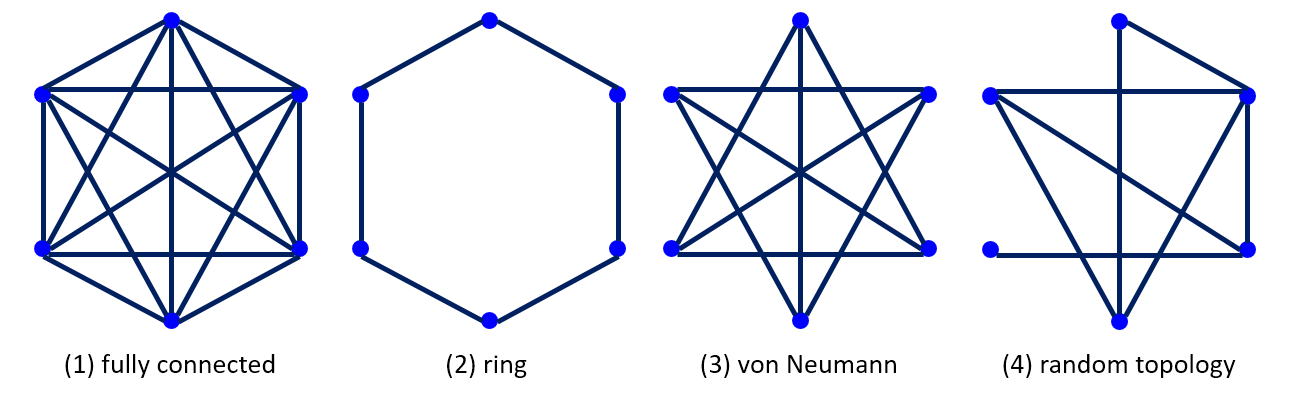
\includegraphics[width=\textwidth]{SPSO_topology}
\caption{Different topologies used by PSO.}\label{fig:SPSO_topology}
\end{figure} 


\subsection{The adaptive random topology} 
The swarm topology defines ``who informs whom" to help distribute the information of optimum solution in the swarm.
Multiple topologies shown in Figure~\ref{fig:SPSO_topology} are adopted in different version of PSO.
The random topology adopted in SPSO 2011 is updated under two circumstances~\cite{Clerc:2012:SPSO2011}:
\begin{itemize}
\item at the very beginning
\item after an iteration with no improvement of the best known fitness value
\end{itemize}

For each particle $p_i$ in a swarm of $n$ particles $S = \{ p_1, p_2, ..., p_n \}$, 
a good topology should allow each $p_i$ to inform itself, 
along with a set of randomly selected particles from the other $n-1$ particles~\cite{Clerc:2007:randomTopology}.
We would like most of the particles to be informed by two to four particles in the topology.
Some of the particles can have no informant except for itself.
There should also exist a non-zero probability for a particle to be informed by all the other particles.

In order to construct a random topology that satisfy the desirable features mentioned above,
Clerc proposed a method~\cite{Clerc:2007:randomTopology} that results in 
a distribution of the sum of $n-1$ independent binary Bernoulli variables, shown in Figure~\ref{fig:SPSO_prob_informant}.
We use the distribution $K=3$, meaning that each particle tells three other particles about their previous best fitness and position.
%The adaptive random topology is formally equivalent to ``Stocastic Star".  
\begin{figure}[!t] \centering
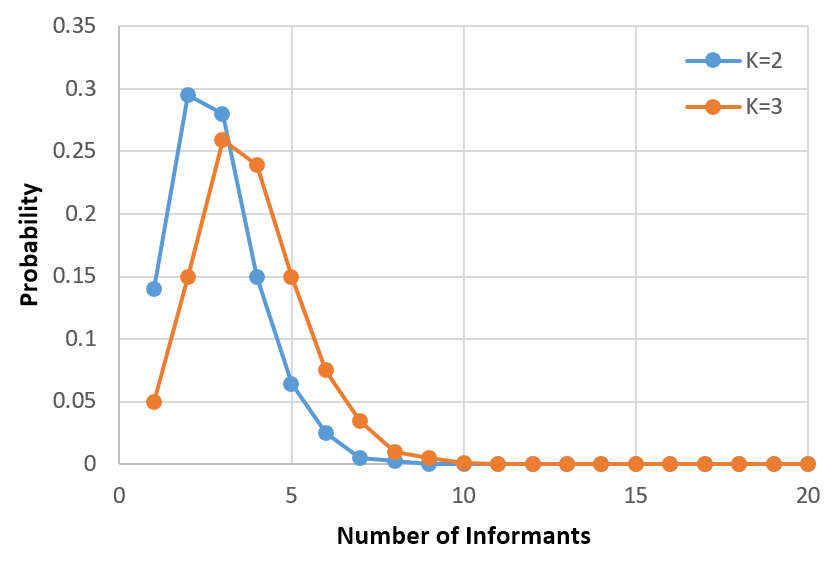
\includegraphics[width=5in]{SPSO_prob_informant}
\caption{Probability of different numbers of informants in the random topology.}\label{fig:SPSO_prob_informant}
\end{figure} 








\section{Ant Colony Optimization for Continuous Domain}


Ant Colony optimization (ACO) is first proposed by Dorigo~\cite{Dorigo:1999:ACO}
to solve combinatorial optimization problems, including scheduling, routing, and timetabling.
These problems aim to find optimal \textit{combinations} or \textit{permutations} of finite sets of available components.
Inspired by the foraging behavior of natural ants, ACO mimics the pheromone deposition of ants along the trail to a food source.
The deposited pheromone, which indicates the quantity and quality of the food, 
creates an indirect communication among ants and enables them to find the shortest paths.
%The pseudo code of ACO is given in Algorithm~\ref{algo:ACO}.
Two major procedures: \textit{solution construction} and \textit{pheromone update}, are detailed in the following paragraph.

\subsection{Discrete solution construction and pheromone update}

\begin{figure}
\centering
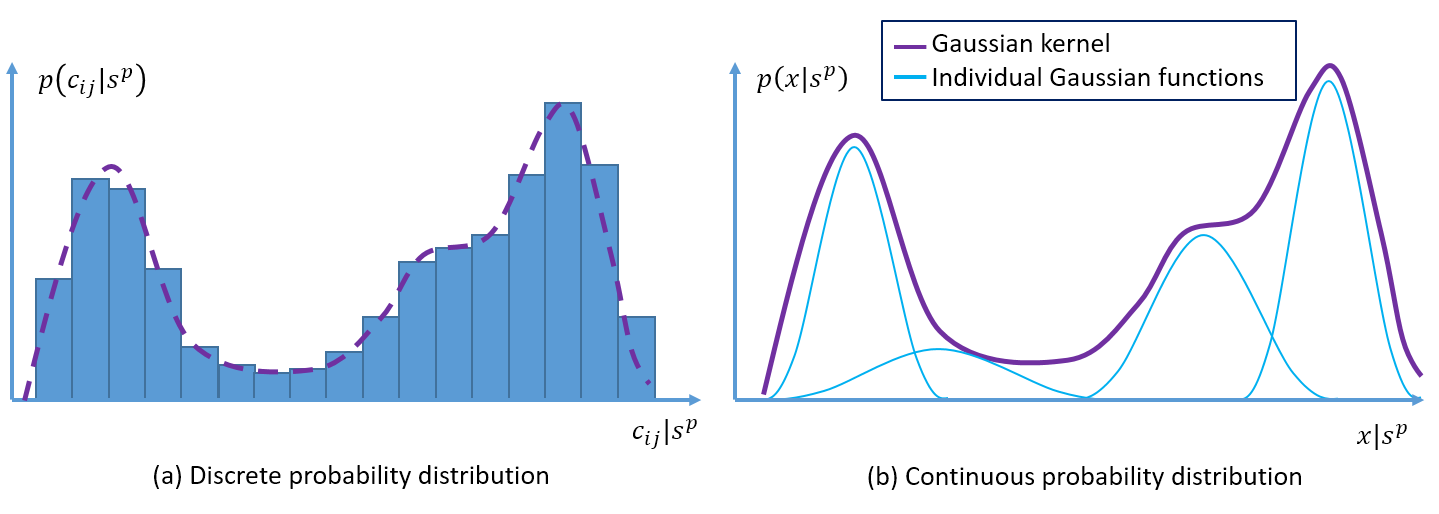
\includegraphics[width=\textwidth]{ACOR_gaussianKernel}
\caption{Comparison of discrete PDF continuous Gaussian kernel PDF.}\label{fig:ACOR_gaussianKernel}
\end{figure}


For \textit{solution construction}, 
we first consider a search space $\boldsymbol{S}$ defined over a finite set of all possible \textit{solution components}, 
denoted by $\boldsymbol{C}$.
Each solution component, denoted by $c_{ij}$, is a decision variable $X_i$ instantiated with value $v^{j}_{i} \in \boldsymbol{D}_i = \{ v^{1}_{i}, ..., v^{|\boldsymbol{D}_i|}_{i}\}$.
To construct a new solution, an artificial ants starts with an empty partial solution $s^{p} = \emptyset$.
During each construction step, the partial solution $s^{p}$ is extended with a feasible solution from the set $N(s^{p}) \in \boldsymbol{C} \setminus s^{p}$.
The probabilistic pheromone model adopted for selecting a feasible solution from $N(s^{p})$ can be defined as follows:

\begin{displaymath}
p(c_{ij}|s^p) = \frac{\tau^{\alpha}_{ij} \cdot \eta(c_{ij})^{\beta}} 
                     {\sum_{c_{i\ell}\in N(s^{p})} \tau^{\alpha}_{i\ell} \cdot \eta(c_{i\ell})^{\beta} },  \forall c_{ij} \in N(s^{p}),
\end{displaymath}
where $\tau_{ij}$ is the pheromone value associated with component $c_{ij}$, and $\eta(\cdot)$ is a weighting function. 
$\alpha$ and $\beta$ are positive parameters which determine the relation between pheromone and heuristic information.

The \textit{pheromone update}, also known as pheromone evaporation, acts as solution selection.
It increases the pheromone values associated with promising solutions and decreases the pheromone values associated to the bad ones.
This is achieved by increasing the pheromone levels of more preferred solutions by $\Delta \tau$.
Let $\rho \in (0,1]$ be the \textit{evaporation rate}.
If the pheromone value is associated with a chosen good solution $s_{ch}$, the pheromone value is updated as following:
\begin{displaymath}
\tau_{ij} = (1 - \rho) \tau_{ij} + \rho \Delta \tau,
\end{displaymath}
while the other unrelated pheromone values are updated as:
\begin{displaymath}
\tau_{ij} = (1 - \rho) \tau_{ij}.
\end{displaymath}
Thus, the discrete pheromone model shown in Figure~\ref{fig:ACOR_gaussianKernel}(a) can be updated to emphasize the good solutions.


\subsection{Continuous solution construction and phermone update}

\begin{figure}
\centering
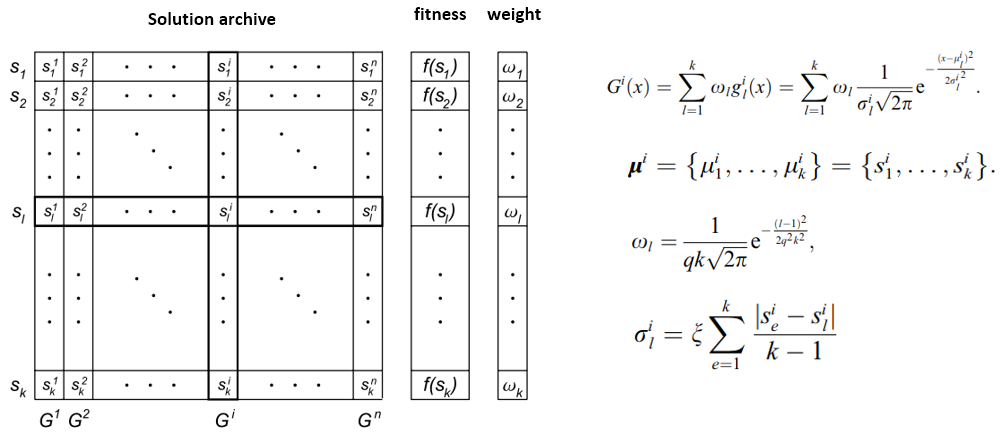
\includegraphics[width=\textwidth]{ACOR_solution_archive}
\caption{The solution archieve of ACO$_R$}\label{fig:ACOR_solution_archive}
\end{figure}

Over the years, multiple approaches of extending the ACO on continuous domain have been given.
One of the most successful version is ACO$_{R}$, proposed by Socha and Dorigo in 2008~\cite{Socha:2008:ACOR}.
It extends ACO to the continuous domain without making any major conceptual change to its structure.
The fundamental idea underlying ACO$_{R}$ is to substitute the discrete probability distribution with a continuous PDF in each dimension, demonstrated in Figure~\ref{fig:ACOR_gaussianKernel}. 
ACO$_R$ keeps a solution archive of \textbf{top-k solutions} it has seen so far, shown in Figure~\ref{fig:ACOR_solution_archive}.
All the solutions are sorted(ties are broken randomly) according to their fitness $f(s)$, 
so that the best solution stays at the top of the archive.
For the $i$-th dimension, a Gaussian kernel PDF $G^i(x)$ is constructed with multiple weighted normal distributions $g_j^i(x)$: 
\begin{displaymath}
G^i(x) = \sum_{j = 1}^{k}\omega_{\ell}g_{\ell}^{i}(x) = 
\sum_{\ell = 1}^{k}\omega_{\ell} \frac{1}{\sigma_{\ell}^{i}\sqrt{2\pi}} e^{-\frac{ (x-\mu^i)^2 }{2 {\sigma^i_\ell}^2}}.
\end{displaymath}
Such a PDF is easy to sample and provides a better flexibility to describe the landscape.
Three elements decide the shape of the Gaussian kernel:
\begin{itemize}
\item $\omega_\ell$ is the \textbf{weight} of the solution $s_\ell$.
\item $\mu^i$ is $i$-th value of all the solutions in the archive.
\item $\sigma^i$ is standard deviation that determines that new samples.
\end{itemize}
Following are some parameters used by ACO$_R$ that also effects the Gaussian kernel construction.
$k$ is the \textit{size of the solution archive}, which works like the memory of the swarm.
It may not be smaller than the number of dimensions.
$q$ represents the \textit{locality} of the search process, \textit{i.e.} how often should we not pick the best solution in the archive.
It controls exploration so that give a higher value of $q$ leads to slower yet more robust convergence.
$\xi > 0$ represents the \textit{speed of convergence} that has effect similar to the \textit{pheromone evaporation} rate in ACO.
It works like selection and enhance the good solutions in the archive.

The initial solution construction process proceed as following.
After evaluating $k$ randomly generates solutions, they are stored along with their fitnesses and weights in the solution archive.
The weights are calculated according to the equation in Figure~\ref{fig:ACOR_solution_archive}.
Then the solution archive is sorted horizontally according to the fitness so that the best solution $s_1$ is on the top

For general \textit{solution construction}, we first define $m$ as the number of ants used in an iteration for sampling.
During each iteration, $m$ new solutions are constructed dimension by dimension by sampling the $i$-th dimension Gaussian kernel $G^i$
A more detailed and efficient process of sampling the Gaussian kernel PDF is described in~\cite{Socha:2008:ACOR}.

\textit{Pheromone update} is accomplished by adding the new samples, their fitness, and the corresponding weight into the archive.
Then, the solution archive is sorted according to the fitness and we only keep the top-k solutions in the archive.
This selection process ensures only the best solutions are kept in the archive.
Therefore, future samples will be constructed near these best solutions and guide the ants toward the optimum.





